% !TEX root = ../main.tex

\section{Use case diagram}
\label{sec:usecase}

\section{Domein class diagram}
\label{sec:domeinclass}

\newpage

\section{Sequentiediagram}
\label{sec:sequentie}

\begin{figure}[H]
  \centering
  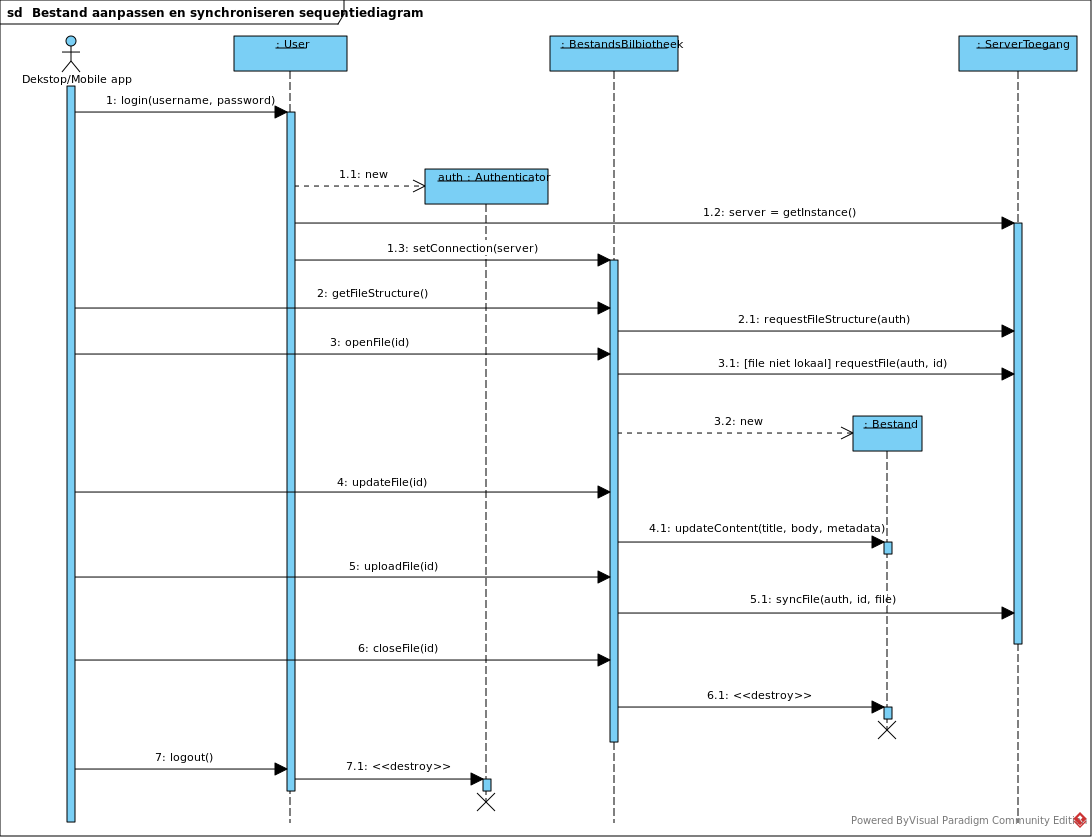
\includegraphics[width=1\textwidth]{images/sequentiediagram.png}
  \label{figure:sequentiediagram}
\end{figure}

\newpage

\section{Activiteitendiagram}
\label{sec:activiteiten}

\begin{figure}[H]
  \centering
  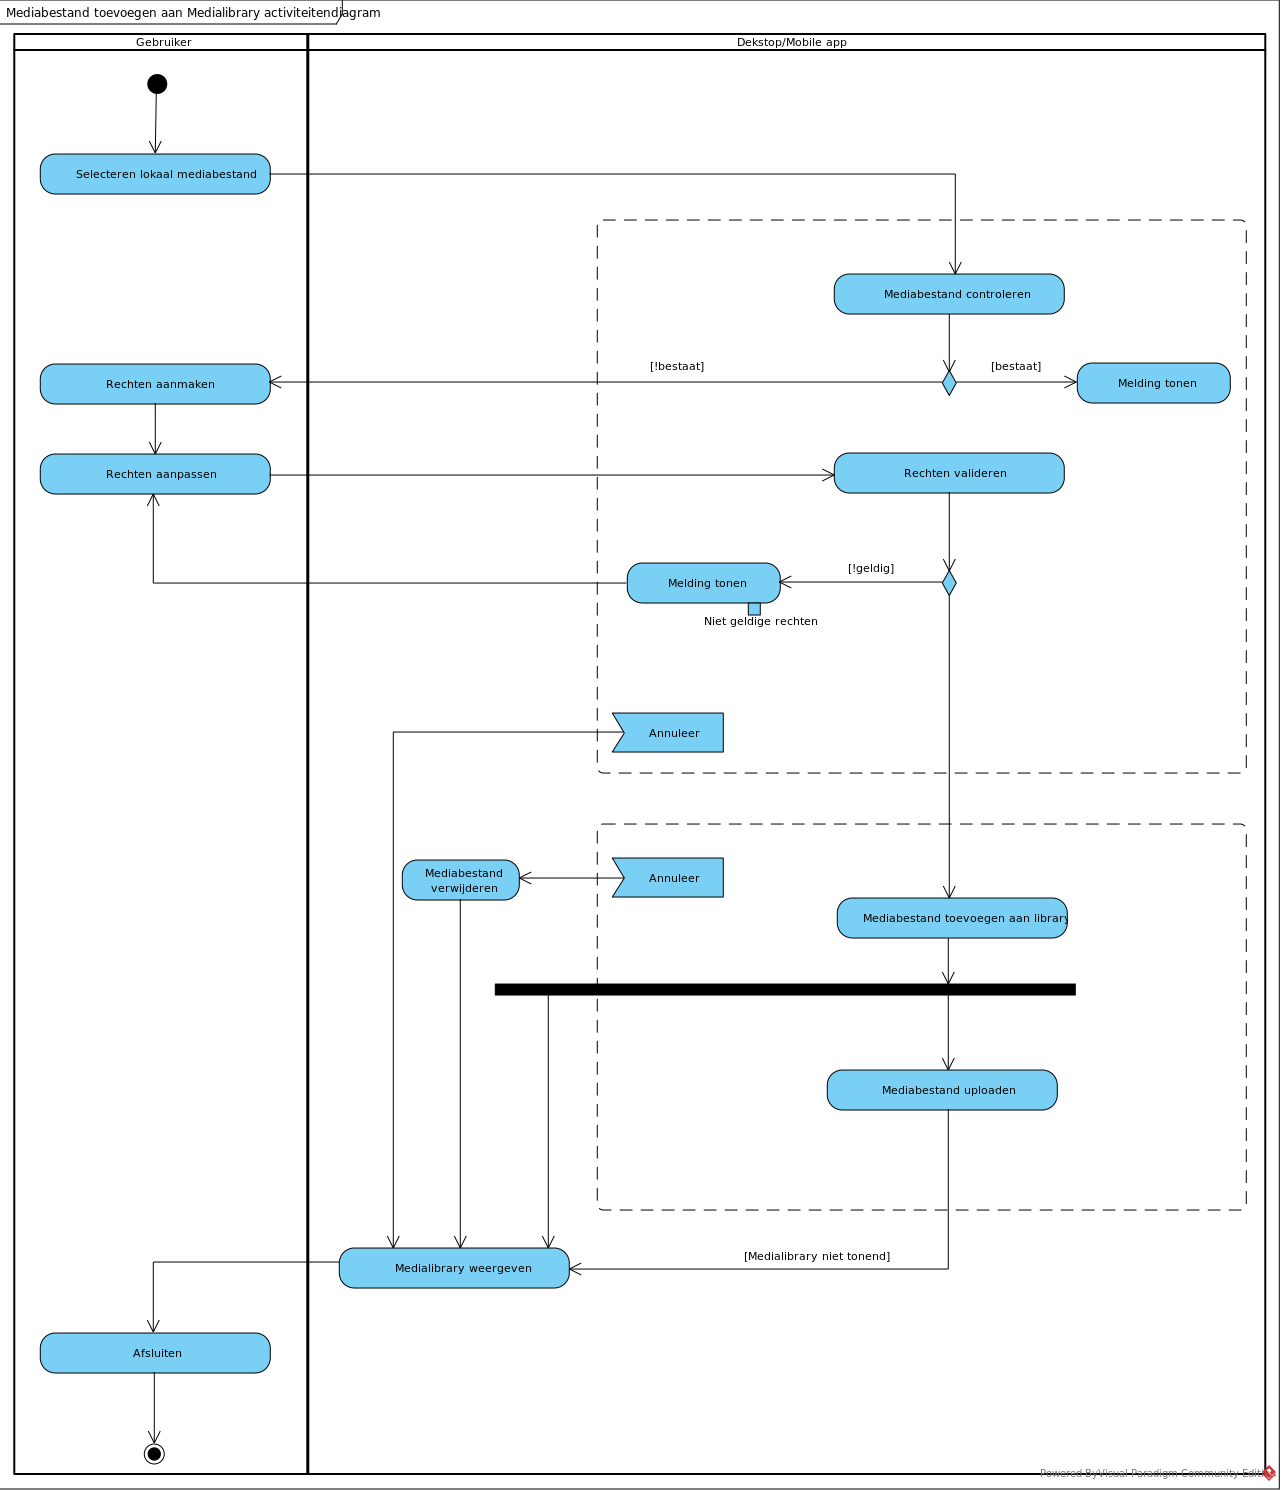
\includegraphics[width=1\textwidth]{images/activiteitendiagram.png}
  \label{figure:activiteitendiagram}
\end{figure}

\newpage

\section{Statemachinediagram}
\label{sec:statemachine}

\begin{figure}[H]
  \centering
  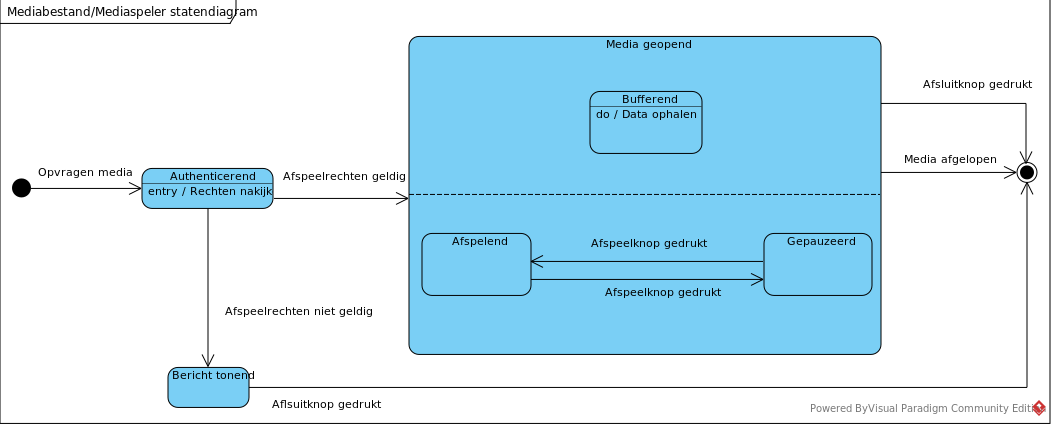
\includegraphics[width=1\textwidth]{images/statendiagram.png}
  \label{figure:statendiagram}
\end{figure}

\newpage

\section{Interactieoverviewdiagram}
\label{sec:interactieoverview}

\begin{figure}[H]
  \centering
  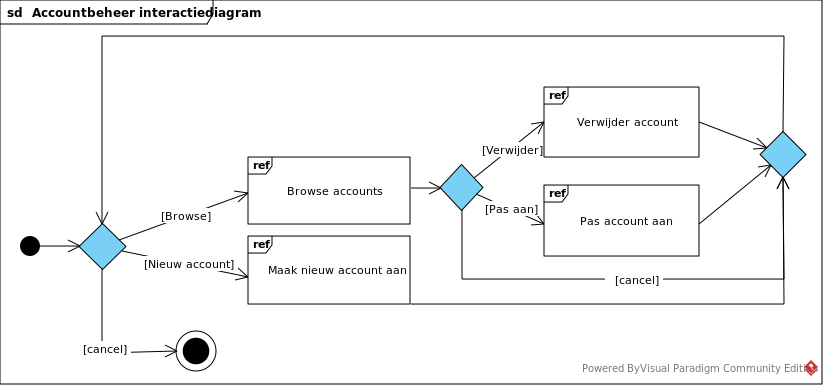
\includegraphics[width=1\textwidth]{images/interactiediagram.png}
  \label{figure:interactiediagram}
\end{figure}
